\section{Absorption into magnons}\label{sec:14.3}

An axion-like particle of mass \SI{10}{\micro eV} has a Compton wavelength $2\pi/m_\phi$ of \SI{12}{cm} and, at the speed $v_E$ of the Earth through the halo (\cref{sec:1.2}), a de Broglie wavelength $2\pi/m_\phi v_E$ of \SI{148}{m}. Across a crystal of centimeter size its gradient is uniform, and through the spin row of \cref{eq:8.1-alp} it acts on every electron spin like one oscillating magnetic field. It brings the momentum $|\vect{p}_\phi| \approx \SI{e-8}{eV}$ and the energy $m_\phi$, and it can be absorbed only by an excitation at vanishing wavevector with energy $m_\phi$. In an ordered magnet that excitation is the uniform precession of the spins. An applied field $\vect{B}_0$ tunes it at \SI{116}{\micro eV} per tesla, which places absorption in ferromagnets and ferrimagnets between a few \si{\micro eV} and about a meV; an antiferromagnet has its uniform mode near \SI{1}{meV} without any field, \SI{1.1}{meV} in MnF$_2$. In both kinds of magnet the rate is a single line, whose weight follows from a conservation law in the first case and from two energies of the spin Hamiltonian in the second.

\subsection{The spin row at vanishing momentum}

With the spin row of \cref{eq:8.1-alp}, the axion-like particle has the coefficient $g^\phi_{s_e,a} = \ii g_{aee}\,p_{\phi,a}/m_e$ per unit amplitude, from $\nabla\phi = \ii\vect{p}_\phi\phi$ for the plane wave. \Cref{eq:8.2-abs} then gives
\begin{equation}
  \varGamma_{\mathrm{abs}} = \frac{g_{aee}^2}{2\omega_\phi m_e^2}\sum_{a,b}p_{\phi,a}\,p_{\phi,b}\,S_{ab}(\vect{p}_\phi,\omega_\phi) ,
  \label{eq:14.3-abs}
\end{equation}
with $a, b$ the Cartesian components of $\vect{s}_e$, as in \cref{eq:7.1-Sfm}. Only the part of $S_{ab}$ symmetric in $a$ and $b$ survives the contraction with $p_{\phi,a}p_{\phi,b}$.

The other rows of the particle create no magnons. The spin current $\mathcal{J}^{\alpha\alpha}_e$ of \cref{eq:8.1-alp}, which carries absorption across an electronic gap (\cref{sec:10.7}), multiplies the polar momentum of each electron by its axial spin and is therefore odd under inversion. Magnons are states of the ground configuration of the magnetic ions, and every multiplet of a configuration has the parity of its orbitals, and $\mathcal{J}^{\alpha\alpha}_e$ therefore has no matrix element between them. It creates charge excitations above the gap of the insulator instead, and reaches magnons only through a crystal field that breaks inversion at the ion together with spin--orbit coupling, which we neglect. The rows of a scalar, $n_e$ and $\mathcal{T}_e$ of \cref{eq:8.1-scalar}, act on the orbital coordinates alone; without spin--orbit coupling they commute with every spin operator, and the scalar has no magnon channel at leading order.

A dark photon reaches the spins through its magnetic field. The electron moment $-(e/m_e)\vect{s}_e$, with $g_e = 2$, couples to $\zeta$ times the field $\vect{B}' = \nabla\times\vect{A}' = \ii\vect{p}_\phi\times\hat{\vect{e}}\,A'$ of a dark photon of polarization $\hat{\vect{e}}$, and the interaction $\zeta(e/m_e)\vect{B}'\cdot\vect{s}_e$ is again the spin row~\cite[Eqs.~(55), (59)]{chigusa2020detecting}. Its coefficient is $g^\phi_{s_e,a} = \ii\zeta e\,(\vect{p}_\phi\times\hat{\vect{e}})_a/m_e$: everything below holds for the dark photon with $g_{aee}\vect{p}_\phi$ replaced by $\zeta e\,\vect{p}_\phi\times\hat{\vect{e}}$. Since $|\vect{B}'| \sim v|\vect{E}'|$, the magnetic coupling is suppressed by the dark-matter speed relative to the electric one and is subleading wherever electric dipoles exist. We write the vacuum $\zeta$. In-medium mixing (\cref{sec:8.4-mixing}) replaces it by $\zeta_{\mathrm{eff}}$, which here depends on the dielectric constant of the magnet and on the conducting surfaces around it, because the wavelength $2\pi/m_\phi$ exceeds the sample. The electric field of the dark photon couples to electric dipoles, and the magnons of a centrosymmetric magnet carry none; magnets in which they do are the multiferroics of \cref{sec:14.5}.

The momentum is small on the scale of the lattice: for YIG, with $a = \SI{12.375}{\angstrom}$, $|\vect{p}_\phi|a = 5\times10^{-11}$ at $m_\phi = \SI{10}{\micro eV}$. To that accuracy $S_{ab}(\vect{p}_\phi,\omega) = S_{ab}(0,\omega)$, the magnetic form factor of \cref{eq:7.1-Fmag} is $F^{\mathrm{mag}}(0) = 1$, and the spin row becomes
\begin{equation}
  \vect{s}_e(0) = \sum_j\lambda_{S,j}\,\vect{S}_j ,
  \label{eq:14.3-s0}
\end{equation}
where $\vect{S}_j$ is the angular momentum that labels the low-energy states of ion $j$ and $\lambda_{S,j}$ is the fraction of it carried by electron spin. For an ion without orbital moment, such as Fe$^{3+}$ and Mn$^{2+}$, $\lambda_S = 1$ and \cref{eq:14.3-s0} is \cref{eq:7.1-Fmag} at $\vect{q} = 0$.

\subsection{The Landé factor}\label{sec:14.3-lande}

In an ion with an open shell, the spin--orbit coupling \cref{eq:3.3-HSO} of each electron, summed over the shell, splits each term of total orbital angular momentum $\vect{L}$ and total spin $\vect{S}$ into multiplets of total angular momentum $\vect{J} = \vect{L} + \vect{S}$. Within one multiplet every vector operator is proportional to $\vect{J}$, by the Wigner--Eckart theorem used in \cref{sec:7.1}, and the constant follows by projecting onto $\vect{J}$: $\vect{S} \to [\langle\vect{S}\cdot\vect{J}\rangle/J(J+1)]\,\vect{J}$, with $\vect{S}\cdot\vect{J} = \frac12(\vect{J}^2 + \vect{S}^2 - \vect{L}^2)$. The electron spin of the ion is therefore
\begin{equation}
  \vect{S} = \lambda_S\,\vect{J}, \qquad
  \lambda_S = \frac{J(J+1) + S(S+1) - L(L+1)}{2J(J+1)} = g_J - 1 ,
  \label{eq:14.3-gJ}
\end{equation}
where the \emph{Landé factor} $g_J$ is defined by the magnetic moment of the multiplet, $\mu_B(\vect{L} + 2\vect{S}) = \mu_B(\vect{J} + \vect{S}) = g_J\mu_B\vect{J}$, so that $g_J = 1 + \lambda_S$~\cite[Eqs.~(30), (34)]{mitridate2020detectability}. The axion-like particle couples to $\lambda_S\vect{J}$ and the dark photon, through $\vect{B}'$, to the moment $(g_J/2)\vect{J}$ in units of $2\mu_B$, the same combination that a magnetic field and a neutron see (\cref{app:C.19}). \Cref{tab:14-lande} lists the ground multiplets of trivalent rare-earth ions, which follow from Hund's rules. Their $4f$ shells sit inside the filled $5s$ and $5p$ shells, so that spin--orbit coupling exceeds the crystal field and $J$ is a good quantum number. For Ce$^{3+}$ and Sm$^{3+}$ the spin points against $\vect{J}$, and in Sm$^{3+}$ the spin coupling exceeds the magnetic one by a factor of five in amplitude. Sm$^{3+}$ is also the most fragile entry: its $J = \frac72$ multiplet lies close above the ground multiplet, and since $g_J = \frac27$ is small, a small admixture changes $\lambda_S/(g_J/2)$ strongly. The crystal field splits the multiplet, but since the projection holds for every state within it, \cref{eq:14.3-gJ} survives the splitting; it fails as soon as the crystal field or exchange admixes a different $J$ multiplet.

\begin{table}[tbp]
  \centering
  \caption{Ground multiplets of trivalent rare-earth ions from Hund's rules: total spin $S$, orbital angular momentum $L$, total angular momentum $J$, Landé factor $g_J$, and the spin fraction $\lambda_S = g_J - 1$ to which an axion-like particle couples (\cref{eq:14.3-gJ}). The last column gives $\lambda_S/(g_J/2)$, the spin coupling relative to the moment that a magnetic field, a neutron and a dark photon see.}
  \label{tab:14-lande}
  \begin{tabular}{@{}lccccrr@{}}
    \toprule
    Ion & $S$ & $L$ & $J$ & $g_J$ & $\lambda_S$ & $\lambda_S/(g_J/2)$ \\
    \midrule
    Ce$^{3+}$ ($4f^1$) & $\frac12$ & 3 & $\frac52$ & $\frac67$ & $-\frac17$ & $-0.33$ \\
    Sm$^{3+}$ ($4f^5$) & $\frac52$ & 5 & $\frac52$ & $\frac27$ & $-\frac57$ & $-5.0$ \\
    Gd$^{3+}$ ($4f^7$) & $\frac72$ & 0 & $\frac72$ & 2 & 1 & 1.0 \\
    Dy$^{3+}$ ($4f^9$) & $\frac52$ & 5 & $\frac{15}2$ & $\frac43$ & $\frac13$ & 0.50 \\
    Er$^{3+}$ ($4f^{11}$) & $\frac32$ & 6 & $\frac{15}2$ & $\frac65$ & $\frac15$ & 0.33 \\
    \bottomrule
  \end{tabular}
\end{table}

The $3d$ ions of most magnetic insulators behave differently. There the crystal field, of energy $\Delta_{\mathrm{CF}}$ of order an eV, exceeds the spin--orbit coupling, and it leaves an orbital ground state $|0\rangle$ that is nondegenerate and can be chosen real. Then $\langle0|\vect{L}|0\rangle = 0$, the orbital moment is quenched, the low-energy states are the $2S + 1$ states of the spin, and the electron spin is $\vect{S}$ itself: $\lambda_S = 1$. Spin--orbit coupling within the term, $\xi_{\mathrm{ion}}\vect{L}\cdot\vect{S}$, admixes excited orbital states $|n\rangle$ at first order, $|0\rangle \to |0\rangle - \sum_n|n\rangle\langle n|\xi_{\mathrm{ion}}\vect{L}\cdot\vect{S}|0\rangle/(E_n - E_0)$. The orbital moment in the admixed state is $\langle L_a\rangle = -2\xi_{\mathrm{ion}}\sum_b\Lambda_{ab}S_b$, with the real symmetric tensor $\Lambda_{ab} = \sum_n\Real\,\langle0|L_a|n\rangle\langle n|L_b|0\rangle/(E_n - E_0)$, so the moment $\vect{L} + 2\vect{S}$ acquires the spectroscopic $g$ tensor of the ion, $g_{\mathrm{ion},ab} = 2\delta_{ab} - 2\xi_{\mathrm{ion}}\Lambda_{ab}$. The shift of $g_{\mathrm{ion}}$ from 2 is of first order in $\xi_{\mathrm{ion}}/\Delta_{\mathrm{CF}}$, while the spin changes only at second order, through the normalization of the admixed state. Setting $\lambda_S = g_{\mathrm{ion}} - 1$ for such an ion would therefore err at first order: for an ion with $g_{\mathrm{ion}} = 2.2$ it gives $\lambda_S = 1.2$ instead of $1 - O(\xi_{\mathrm{ion}}^2/\Delta_{\mathrm{CF}}^2)$, and a rate too large by 1.44. The rule $\lambda_S = g_J - 1$ belongs to $J$ multiplets only. The spectroscopic $g_{\mathrm{ion}}$ of a quenched ion converts a measured magnetic response into the spin response, the conversion that \cref{sec:14.4} applies to neutron data.

\subsection{The Larmor line}\label{sec:14.3-larmor}

Take a magnet with rotation-invariant exchange, such as the Heisenberg model \cref{eq:7.1-heis}, in a uniform field, and give all ions the same $\lambda_S$ and the same spectroscopic factor $g_{\mathrm{ion}}$. We take $\hat{\vect{z}}$ along the net spin, which the field selects opposite to itself because the electron moment is opposite to its spin, so that the Zeeman energy is $-\omega_{\mathrm{Lar}}S^z_{\mathrm{tot}}$ with the Larmor frequency $\omega_{\mathrm{Lar}} = g_{\mathrm{ion}}\mu_B|\vect{B}_0|$, \SI{115.8}{\micro eV} or \SI{28.0}{GHz} per tesla for $g_{\mathrm{ion}} = 2$. The total spin $\vect{S}_{\mathrm{tot}} = \sum_j\vect{S}_j$ commutes with the exchange, and the Zeeman term leads to $[H, S^-_{\mathrm{tot}}] = \omega_{\mathrm{Lar}}S^-_{\mathrm{tot}}$. Acting on any eigenstate, $S^-_{\mathrm{tot}}$ therefore produces an eigenstate exactly $\omega_{\mathrm{Lar}}$ higher, however strong and complicated the exchange, and $S^+_{\mathrm{tot}}$ one exactly $\omega_{\mathrm{Lar}}$ lower~\cite[Eqs.~(2.4), (2.5)]{oshikawa2002electron}. By \cref{eq:14.3-s0}, $\vect{s}_e(0) = \lambda_S\vect{S}_{\mathrm{tot}}$, and all of $S_{ab}(0,\omega)$ sits at $\omega = \pm\omega_{\mathrm{Lar}}$ (and at $\omega = 0$ for $S^z_{\mathrm{tot}}$, which is conserved).

The weight follows from the spin algebra. In \cref{eq:4.2-Sab}, the line at $+\omega_{\mathrm{Lar}}$ comes from the $S^-_{\mathrm{tot}}$ parts of $s_{e,x} = \lambda_S(S^+_{\mathrm{tot}} + S^-_{\mathrm{tot}})/2$ and $s_{e,y} = \lambda_S(S^+_{\mathrm{tot}} - S^-_{\mathrm{tot}})/2\ii$, and its strength is the thermal average $\langle S^+_{\mathrm{tot}}S^-_{\mathrm{tot}}\rangle$. The commutator gives $\langle S^+_{\mathrm{tot}}S^-_{\mathrm{tot}}\rangle - \langle S^-_{\mathrm{tot}}S^+_{\mathrm{tot}}\rangle = 2\langle S^z_{\mathrm{tot}}\rangle$, and detailed balance for a transition of energy $\omega_{\mathrm{Lar}}$ gives $\langle S^-_{\mathrm{tot}}S^+_{\mathrm{tot}}\rangle = \ee^{-\beta\omega_{\mathrm{Lar}}}\langle S^+_{\mathrm{tot}}S^-_{\mathrm{tot}}\rangle$. With $\mathfrak{s}_{\mathrm{net}} = \langle S^z_{\mathrm{tot}}\rangle/N$ the net spin per unit cell of volume $\Omega$, $N$ cells and $\Vol = N\Omega$:
\begin{keyresult}[The Larmor line]
\begin{equation}
  S_{ab}(0,\omega) = \frac{\pi\lambda_S^2\,\mathfrak{s}_{\mathrm{net}}}{\Omega}\,\frac{\delta_{ab} - \hat z_a\hat z_b + \ii\epsilon_{abc}\hat z_c}{1 - \ee^{-\beta\omega_{\mathrm{Lar}}}}\,\delta(\omega - \omega_{\mathrm{Lar}}) ,
  \label{eq:14.3-larmor}
\end{equation}
for $\omega > 0$, and in \cref{eq:14.3-abs}
\begin{equation}
  \varGamma_{\mathrm{abs}} = \frac{\pi g_{aee}^2\lambda_S^2\,\mathfrak{s}_{\mathrm{net}}\,p_{\phi\perp}^2}{2m_e^2\,\omega_\phi\,\Omega}\,\frac{\delta(\omega_\phi - \omega_{\mathrm{Lar}})}{1 - \ee^{-\beta\omega_{\mathrm{Lar}}}} ,
  \label{eq:14.3-rate}
\end{equation}
with $p_{\phi\perp}^2 = |\vect{p}_\phi|^2 - (\vect{p}_\phi\cdot\hat{\vect{z}})^2$, for exchange invariant under spin rotations and uniform $\lambda_S$ and $g_{\mathrm{ion}}$, at any temperature.
\end{keyresult}
At $T = 0$ and with $\mathfrak{s}_{\mathrm{net}} \to |\vect{S}|$, \cref{eq:14.3-larmor} is the one-magnon response \cref{eq:7.1-Sfm} of the ferromagnet at $\vect{q}_r = 0$, now shown to hold beyond linear spin-wave theory. It holds for a ferrimagnet, whose net spin is the difference of its sublattices, and for a paramagnet, whose $\mathfrak{s}_{\mathrm{net}}$ is the magnetization induced by the field. The counted rate carries $1/(1 - \ee^{-\beta\omega_{\mathrm{Lar}}})$; the net rate $\varGamma_{\mathrm{net}}$ of \cref{eq:8.2-abs} carries $\mathfrak{s}_{\mathrm{net}}$ alone. With one sublattice and $\lambda_S = 1$, \cref{eq:14.3-rate} is the rate of Refs.~\cites[Eqs.~(27), (35)]{mitridate2020detectability}[Eqs.~(25)--(27)]{chigusa2020detecting}.

The Larmor line is also a selection rule. YIG has 20 magnetic ions in its primitive cell and 20 magnon branches; 19 of them are gapped at $\vect{k} = 0$, and \cref{eq:14.3-larmor} leaves them no weight. In classical terms, a uniform field $\vect{f}$ that precesses every spin alike changes no exchange energy, $\dd(\vect{S}_j\cdot\vect{S}_{j'})/\dd t \propto (\vect{f}_j - \vect{f}_{j'})\cdot(\vect{S}_j\times\vect{S}_{j'})$~\cite[Eq.~(28)]{mitridate2020detectability}. The commutator states the same thing exactly. It also shows what lifts the rule. If $\lambda_{S,j}$ differs between sublattices, $\vect{s}_e(0)$ is no longer proportional to $\vect{S}_{\mathrm{tot}}$, and the gapped branches acquire weight in proportion to $(\lambda_{S,j} - \lambda_{S,j'})^2$; anisotropic exchange or single-ion anisotropy breaks the commutation of $\vect{S}_{\mathrm{tot}}$ with $H$ and moves the uniform line away from $\omega_{\mathrm{Lar}}$.

\Cref{eq:14.3-rate} has a delta function, and a real line has a width. The width of the field itself is $\sim m_\phi v_0^2$, a fraction $6\times10^{-7}$ of $m_\phi$, set by the coherence time $t_{\mathrm{coh}} = 1/m_\phi v_0^2$ of \cref{sec:8.2-absorption}, \SI{0.10}{ms} at \SI{10}{\micro eV}. The uniform mode of a good magnet is broader. For the uniform mode of YIG (the Kittel mode of \cref{sec:14.3-kittel}) we take the full width $\varGamma_{\mathrm{M}} = 10^{-5}\omega$ assumed in Ref.~\cite[Sect.~V\,B]{mitridate2020detectability}, not a millikelvin measurement. The delta function then becomes a Lorentzian of full width $\varGamma_{\mathrm{M}}$, whose peak is $2/\pi\varGamma_{\mathrm{M}}$. Averaging $p_{\phi\perp}^2 = m_\phi^2v_\perp^2$ over the halo and multiplying by $\rho_\chi/m_\phi\rho_T$, the event rate per unit target mass on resonance at $T \to 0$ is
\begin{equation}
  \mathcal{R}_{\mathrm{peak}} = \frac{\rho_\chi\,g_{aee}^2\,\langle v_\perp^2\rangle\,\lambda_S^2\,\mathfrak{s}_{\mathrm{net}}}{m_e^2\,\rho_T\Omega\,\varGamma_{\mathrm{M}}} ,
  \label{eq:14.3-peak}
\end{equation}
where $\rho_T\Omega$ is the mass of the unit cell. The boson mass has dropped out except through $\varGamma_{\mathrm{M}}$. For the standard halo, $\langle v_\perp^2\rangle = v_0^2 + |\vect{v}_E|^2\sin^2\theta_E$, with $\theta_E$ the angle between $\hat{\vect{z}}$ and the velocity of the Earth through the halo, and the rate is modulated daily by up to a factor $0.47$ as the laboratory rotates (\cref{sec:1.2}). The golden-rule mean needs an exposure long compared with the shorter of $t_{\mathrm{coh}}$ and $1/\varGamma_{\mathrm{M}}$, and a single record matches it only beyond $t_{\mathrm{coh}}$ (\cref{sec:14.6-regime}); for shorter exposures the field drives the mode coherently, which \cref{sec:14.6} treats. The exchange dispersion of the mode, $\omega = \omega_{\mathrm{Lar}} + k^2/2M_{\mathrm{sw}}$ with $M_{\mathrm{sw}} = 1/2D_{\mathrm{sw}} = \SI{3.25}{MeV}$ for the stiffness of YIG in \cref{we:14-hybrid}, shifts the line by $10^{-18}$ of $m_\phi$ at $k = m_\phi v_E$. The same line also absorbs the energy that exothermic dark matter releases when its splitting $|\Delta_\chi|$ matches $\omega_{\mathrm{Lar}}$, a channel common to phonons, magnons and plasmons (\cref{sec:17.3}).

\subsection{The Kittel mode and demagnetizing fields}\label{sec:14.3-kittel}

A magnetized body produces its own field, and the Larmor line assumes there is none. A uniformly magnetized ellipsoid has a uniform internal field: in Heaviside--Lorentz units with $\mu_0 = 1$ it is $\vect{B}_0 - \mathsf{N}\vect{M}$, where the demagnetizing tensor $\mathsf{N}$ is diagonal along the axes of the ellipsoid with elements $N^{\mathrm{dm}}_x + N^{\mathrm{dm}}_y + N^{\mathrm{dm}}_z = 1$. A sphere has $N^{\mathrm{dm}}_i = \frac13$, a thin film $N^{\mathrm{dm}} = 1$ along its normal and 0 in its plane. The field adds the magnetostatic energy $\frac12\Vol\sum_iN^{\mathrm{dm}}_iM_i^2$, and in the magnet of \cref{sec:14.3-larmor} the magnetization is $\vect{M} = 2\mu_B\vect{S}_{\mathrm{tot}}/\Vol$ for $g_{\mathrm{ion}} = 2$. Let $\vect{B}_0$ and the net spin lie along the $z$ axis of the ellipsoid. To second order in the transverse components, with $S^z_{\mathrm{tot}} = S_{\mathrm{tot}} - (S_{\mathrm{tot},x}^2 + S_{\mathrm{tot},y}^2)/2S_{\mathrm{tot}}$, the energy of the uniform mode is
\begin{equation}
  H_{\mathrm{u}} = \frac{1}{2S_{\mathrm{tot}}}\Bigl[\omega_{\mathrm{Kit},x}\,S_{\mathrm{tot},x}^2 + \omega_{\mathrm{Kit},y}\,S_{\mathrm{tot},y}^2\Bigr], \qquad
  \omega_{\mathrm{Kit},i} = \omega_{\mathrm{Lar}} + \bigl(N^{\mathrm{dm}}_i - N^{\mathrm{dm}}_z\bigr)\,\omega_M ,
  \label{eq:14.3-Hu}
\end{equation}
where $\omega_M = 2\mu_BM_{\mathrm{s}}$ is the saturation magnetization $M_{\mathrm{s}} = |\vect{M}|$ in units of frequency ($2\mu_B\mu_0M_{\mathrm{s}}$ in SI units) and $S_{\mathrm{tot}} = N\mathfrak{s}_{\mathrm{net}}$. With the Holstein--Primakoff form of \cref{eq:7.1-HP} for the total spin, $S_{\mathrm{tot},x} = S_{\mathrm{tot}}^{1/2}\hat x$ and $S_{\mathrm{tot},y} = S_{\mathrm{tot}}^{1/2}\hat p$, where $\hat x = (a_0 + a_0^\dagger)/\sqrt2$ and $\hat p = -\ii(a_0 - a_0^\dagger)/\sqrt2$ obey $[\hat x, \hat p] = \ii$. \Cref{eq:14.3-Hu} is then an oscillator $\frac12(\omega_{\mathrm{Kit},x}\hat x^2 + \omega_{\mathrm{Kit},y}\hat p^2)$, whose frequency is the Kittel formula~\cite{kittel1948theory}
\begin{equation}
  \omega_{\mathrm{Kit}} = \bigl(\omega_{\mathrm{Kit},x}\,\omega_{\mathrm{Kit},y}\bigr)^{1/2} .
  \label{eq:14.3-kittel}
\end{equation}
In its ground state $\langle\hat x^2\rangle = \frac12(\omega_{\mathrm{Kit},y}/\omega_{\mathrm{Kit},x})^{1/2}$, so the transverse weights of \cref{eq:14.3-larmor} become elliptical, $|\langle1|S_{\mathrm{tot},x}|0\rangle|^2 = \frac12S_{\mathrm{tot}}(\omega_{\mathrm{Kit},y}/\omega_{\mathrm{Kit},x})^{1/2}$ and $|\langle1|S_{\mathrm{tot},y}|0\rangle|^2 = \frac12S_{\mathrm{tot}}(\omega_{\mathrm{Kit},x}/\omega_{\mathrm{Kit},y})^{1/2}$. In \cref{eq:14.3-rate} this replaces $\delta(\omega_\phi - \omega_{\mathrm{Lar}})$ by $\delta(\omega_\phi - \omega_{\mathrm{Kit}})$ and $p_{\phi\perp}^2$ by
\begin{equation}
  p_{\phi,x}^2\Bigl(\frac{\omega_{\mathrm{Kit},y}}{\omega_{\mathrm{Kit},x}}\Bigr)^{1/2} + p_{\phi,y}^2\Bigl(\frac{\omega_{\mathrm{Kit},x}}{\omega_{\mathrm{Kit},y}}\Bigr)^{1/2} .
  \label{eq:14.3-ellipse}
\end{equation}
Averaged over transverse directions of $\vect{p}_\phi$, the weight grows by $(\omega_{\mathrm{Kit},x} + \omega_{\mathrm{Kit},y})/2\omega_{\mathrm{Kit}} \ge 1$. The sum of the two transverse weights is not conserved by the shape, and the line moves; the Larmor theorem fails because the magnetostatic energy is not invariant under a rotation of $\vect{S}_{\mathrm{tot}}$.

For a sphere every $N^{\mathrm{dm}}_i$ is equal, and $\omega_{\mathrm{Kit}} = \omega_{\mathrm{Lar}}$ with circular weights: the Larmor line survives. A thin film with $\vect{B}_0$ in its plane has $\omega_{\mathrm{Kit}} = [\omega_{\mathrm{Lar}}(\omega_{\mathrm{Lar}} + \omega_M)]^{1/2}$, and with $\vect{B}_0$ along its normal $\omega_{\mathrm{Kit}} = \omega_{\mathrm{Lar}} - \omega_M$. All of this assumes a body saturated along $\vect{B}_0$, which needs an internal field $|\vect{B}_0| - N^{\mathrm{dm}}_zM_{\mathrm{s}} > 0$; below it the sample breaks into domains and \cref{eq:14.3-Hu} does not apply. A uniaxial anisotropy field $B_A$ along $\vect{B}_0$ adds $g_{\mathrm{ion}}\mu_BB_A$ to both $\omega_{\mathrm{Kit},i}$, moving the line without changing its weights.

Beyond the uniform field of an ellipsoid, the dipolar interaction couples the precession at different points of the sample and produces the magnetostatic modes of finite wavevector. The dark-matter field is uniform over the sample, since $1/m_\phi v \gg$ its size, and in an ellipsoid it drives the Kittel mode alone; in a body of any other shape the internal field is nonuniform and the weight spreads over several magnetostatic modes. The limits $\vect{k} \to 0$ and sample size $\to\infty$ do not commute: the mode at $\vect{k} \to 0$ in an infinite crystal has no demagnetizing field along $\vect{k}$, while the uniform mode of any finite body has the field of its shape. Absorption needs the second. \Cref{lim:14.3a}a compares the Larmor line with the film.

\begin{workedexample}{The Kittel-mode rate of YIG for a \SI{10}{\micro eV} axion-like particle}\label{we:14-yig}
YIG, Y$_3$Fe$_5$O$_{12}$, has a body-centered cubic lattice with $a = \SI{12.375}{\angstrom}$~\cite{nakatsuka1995site} and a primitive cell of volume $\Omega = a^3/2 = \SI{947.6}{\angstrom^3}$ that holds four formula units, of mass $\rho_T\Omega = \SI{2951.8}{u}$. Its 20 Fe$^{3+}$ ions, each with $|\vect{S}| = \frac52$ and no orbital moment, order as a ferrimagnet, 12 against 8~\cite[Sect.~III]{mitridate2020detectability}, so that $\mathfrak{s}_{\mathrm{net}} = 4\times\frac52 = 10$ and $\lambda_S = 1$. The saturation magnetization is $M_{\mathrm{s}} = 20\mu_B/\Omega$, $\mu_0M_{\mathrm{s}} = \SI{0.246}{T}$, or \SI{37.8}{emu/g}, close to the measured \SI{38}{emu/g} at \SI{0.1}{K}~\cite{chigusa2020detecting}; then $\omega_M = \SI{28.5}{\micro eV}$. (The model of \cref{we:14-hybrid} used the room-temperature $4\pi M_{\mathrm{s}} = \SI{1750}{G}$; at low temperature it is \SI{2460}{G}.)

\emph{Field.} Since in a sphere the line sits at $\omega_{\mathrm{Lar}}$, $m_\phi = \SI{10}{\micro eV}$ needs $|\vect{B}_0| = m_\phi/2\mu_B = \SI{86.4}{mT}$. The sphere saturates for $|\vect{B}_0| > \mu_0M_{\mathrm{s}}/3 = \SI{82.0}{mT}$, that is for lines above \SI{9.49}{\micro eV}; at \SI{10}{\micro eV} the internal field is only \SI{4.4}{mT}. At \SI{10}{mK}, $\beta m_\phi = 11.6$ and the thermal factor of \cref{eq:14.3-rate} is $1 + 9\times10^{-6}$.

\emph{Rate.} The assumed width is $\varGamma_{\mathrm{M}} = 10^{-5}m_\phi = \SI{1.0e-10}{eV}$, a full width of \SI{24}{kHz}, with $1/\varGamma_{\mathrm{M}} = \SI{6.6}{\micro s}$. With $\rho_\chi = \SI{0.3}{GeV.cm^{-3}}$, $\hat{\vect{z}}$ perpendicular to $\vect{v}_E$, so that $\langle v_\perp^2\rangle = v_0^2 + v_E^2 = 1.33\times10^{-6}$, and $g_{aee} = 10^{-13}$, \cref{eq:14.3-peak} gives
\begin{equation*}
  \mathcal{R}_{\mathrm{peak}} = \SI{3.63}{s^{-1}.kg^{-1}} = \SI{1.15e8}{kg^{-1}.yr^{-1}} .
\end{equation*}
A sphere \SI{1}{cm} across, of \SI{2.7}{g}, would absorb 35 particles an hour while its line sits on $m_\phi$, within \SI{24}{kHz}. With $\hat{\vect{z}}$ along $\vect{v}_E$ the rate falls to 0.47 of this value.

\emph{Shape.} A thin film with the field in its plane reaches \SI{10}{\micro eV} at $\omega_{\mathrm{Lar}} = \SI{3.16}{\micro eV}$, $|\vect{B}_0| = \SI{27.3}{mT}$, and it is saturated at any field. By \cref{eq:14.3-ellipse} the component of $\vect{p}_\phi$ in the plane of the film counts 3.16 times and the normal one 0.316 times; averaged, the rate is 1.74 times that of the sphere.
\end{workedexample}

\subsection{Antiferromagnetic resonance}\label{sec:14.3-afmr}

An antiferromagnet has no net spin, $\mathfrak{s}_{\mathrm{net}} = 0$ in zero field, and the Larmor line of \cref{eq:14.3-larmor} is empty. With isotropic exchange the uniform mode is the Goldstone mode at $\omega = 0$, and \cref{eq:7.1-weights} assigns it a weight that vanishes linearly in $k$. Anisotropy changes both. Take two sublattices, A along $+\hat{\vect{z}}$ and B along $-\hat{\vect{z}}$, with an easy axis along $\hat{\vect{z}}$. The uniform mode then depends on two energies, written as frequencies. The exchange frequency $\omega_E = |\vect{S}|J^{\mathrm{ex}}_{\mathrm{AB}}(0)$ is the cost of one deviation in the exchange field of the other sublattice, and the anisotropy frequency $\omega_A$ is the cost of one deviation away from the easy axis. In fields, $\omega_E = g_{\mathrm{ion}}\mu_BB_E$ and $\omega_A = g_{\mathrm{ion}}\mu_BB_A$. At $\vect{k} = 0$ the bosonic Hamiltonian \cref{eq:7.1-Hk} has $|\vect{S}|A_0 = \omega_E + \omega_A$ and $|\vect{S}|B_0 = \omega_E$, since the intra-sublattice terms cancel at $\vect{k} = 0$ and the anisotropy adds only to the diagonal. \Cref{eq:7.1-afm} then gives the two degenerate modes at
\begin{equation}
  \omega_{\mathrm{AFMR}} = \bigl[(\omega_E + \omega_A)^2 - \omega_E^2\bigr]^{1/2} = \bigl[\omega_A(2\omega_E + \omega_A)\bigr]^{1/2} ,
  \label{eq:14.3-afmr}
\end{equation}
the frequency of \emph{antiferromagnetic resonance}, the geometric mean of the anisotropy frequency and twice the exchange frequency. Its large size is the exchange enhancement already seen in the linear dispersion of \cref{sec:7.1}: a uniform tilt of one sublattice drags the other through the pair term, and the precession works against the full exchange field.

The weight is \cref{eq:7.1-weights} at $\vect{k} = 0$. In the uniform transverse spin $S^x_{\mathrm{tot}} = (|\vect{S}|N_{\mathrm{s}}/2)^{1/2}(d_{\mathrm{A}0} + d^\dagger_{\mathrm{A}0} + d_{\mathrm{B}0} + d^\dagger_{\mathrm{B}0})$, the inverse of \cref{eq:7.1-bogo} gives $d_{\mathrm{A}0} + d^\dagger_{\mathrm{B}0} = (u^{\mathrm{M}}_0 - v^{\mathrm{M}}_0)(a_{01} + a^\dagger_{02})$, and each mode is created with the amplitude $(|\vect{S}|N_{\mathrm{s}}/2)^{1/2}(u^{\mathrm{M}}_0 - v^{\mathrm{M}}_0)$. Summed over the two modes and divided by the number $N_{\mathrm{s}}$ of antiparallel pairs, with $(u^{\mathrm{M}}_0 - v^{\mathrm{M}}_0)^2 = (A_0 - B_0)/(A_0^2 - B_0^2)^{1/2} = \omega_A/\omega_{\mathrm{AFMR}}$:
\begin{keyresult}[Uniform weight of a two-sublattice antiferromagnet]
\begin{equation}
  \frac{1}{N_{\mathrm{s}}}\sum_{\nu=1,2}\bigl|\langle\nu|S^x_{\mathrm{tot}}|0\rangle\bigr|^2 = |\vect{S}|\,\frac{\omega_{\mathrm{AFMR}}}{2\omega_E + \omega_A} \;\simeq\; |\vect{S}|\Bigl(\frac{\omega_A}{2\omega_E}\Bigr)^{1/2} \quad (\omega_A \ll \omega_E),
  \label{eq:14.3-afmrweight}
\end{equation}
at linear spin-wave order and $T = 0$, against $|\vect{S}|$ for a ferromagnetic pair. In \cref{eq:14.3-rate} the antiferromagnet at $\vect{B}_0 = 0$ enters with $\mathfrak{s}_{\mathrm{net}} \to 2|\vect{S}|\omega_{\mathrm{AFMR}}/(2\omega_E + \omega_A)$ per pair cell, $\delta(\omega_\phi - \omega_{\mathrm{Lar}}) \to \delta(\omega_\phi - \omega_{\mathrm{AFMR}})$ and $\ii\epsilon_{abc}\hat z_c \to 0$.
\end{keyresult}
The same factor $\omega_{\mathrm{AFMR}}/(2\omega_E + \omega_A)$ that raises the frequency suppresses the weight, so the product of the two is the anisotropy frequency $\omega_A$: an antiferromagnet trades rate for reach. The two modes carry opposite circular polarizations, one lowering and one raising $S^z_{\mathrm{tot}}$ (\cref{sec:7.1}), and their contributions to $\ii\epsilon_{abc}$ cancel. A field along the easy axis adds $\mp g_{\mathrm{ion}}\mu_B|\vect{B}_0|$ to the diagonal energies of the two modes. Since it couples to the conserved $S^z_{\mathrm{tot}}$, it commutes with the Bogoliubov transformation, and the line splits into $\omega_{\mathrm{AFMR}} \pm g_{\mathrm{ion}}\mu_B|\vect{B}_0|$ with both weights unchanged, up to the spin-flop field $B_{\mathrm{sf}} = [B_A(2B_E - B_A)]^{1/2}$, where the lower mode has fallen to \SI{0.01}{meV} in MnF$_2$ and the sublattices turn perpendicular to the field. Shape enters only through the small net moment of the precession, and it shifts $\omega_{\mathrm{AFMR}}$ by a fraction of order $\omega_M/\omega_E$, $1.6\times10^{-2}$ in MnF$_2$ with $\omega_M$ formed from the sublattice magnetization, $\mu_0M = \SI{0.74}{T}$. A ferrimagnet such as YIG has modes of both kinds. Besides its Larmor line, its 19 gapped branches at $\vect{k} = 0$ are exchange modes in which the sublattices precess against each other. With uniform $\lambda_S$ and isotropic exchange their weight is the zero found in \cref{sec:14.3-larmor}.

The exchange and anisotropy frequencies are measured by neutron scattering and magnetic resonance, or computed by DFT~$+\,U$ with the energy-mapping methods of \cref{sec:14.1}. MnF$_2$ is the standard two-sublattice antiferromagnet: Mn$^{2+}$ ions with $|\vect{S}| = \frac52$ and no orbital moment, $\lambda_S = 1$, one antiparallel pair per rutile cell of mass \SI{185.9}{u}, and an easy axis along $c$ set mainly by the dipolar interaction~\cite{bayrakci2013lifetimes}. Neutron scattering finds a zone-center gap of \SI{1.1}{meV} at \SI{4}{K}~\cite{bayrakci2013lifetimes}, and the spin flop occurs near \SI{9.4}{T}~\cite[Fig.~1]{vaidya2020subterahertz}. Since $\omega_{\mathrm{AFMR}} \simeq g_{\mathrm{ion}}\mu_BB_{\mathrm{sf}}$ for $\omega_A \ll \omega_E$, the two measurements agree with each other: \SI{1.1}{meV} corresponds to \SI{9.5}{T}. The exchange and anisotropy fields fitted by Vaidya and collaborators, $B_E = \SI{47.05}{T}$ and $B_A = \SI{0.82}{T}$~\cite{vaidya2020subterahertz}, give $\omega_E = \SI{5.447}{meV}$ and $\omega_A = \SI{0.0949}{meV}$, and \cref{eq:14.3-afmr} gives $\omega_{\mathrm{AFMR}} = \SI{1.021}{meV}$ (\SI{247}{GHz}) with $B_{\mathrm{sf}} = \SI{8.75}{T}$, both \SI{7}{\percent} below the measured pair. The weight factor is $0.0929$, within half a percent of $(\omega_A/2\omega_E)^{1/2} = 0.0933$, and a pair absorbs with $0.232$ against 2.5 for a ferromagnetic pair, 0.74 of the weight of YIG per unit mass. With the same assumed ratio $\varGamma_{\mathrm{M}}/\omega = 10^{-5}$, the peak rate \cref{eq:14.3-peak} at the resonance is $7.2\times10^{-3}$ of that of YIG at \SI{10}{\micro eV}, \SI{2.6e-2}{s^{-1}.kg^{-1}} for $g_{aee} = 10^{-13}$, unchanged if $\omega_A$ is fitted to the measured gap instead: the rate goes as $|\vect{S}|\omega_A/\omega_{\mathrm{AFMR}}^2$, because $\varGamma_{\mathrm{M}}$ grows with the frequency. A field along $c$ sweeps the lower line from \SI{1.1}{meV} nearly to zero at the spin flop (\cref{fig:14-lines}), and one crystal covers every mass below \SI{1}{meV} with a weight that stays the same along the sweep.

\begin{figure}[tbp]
  \centering
  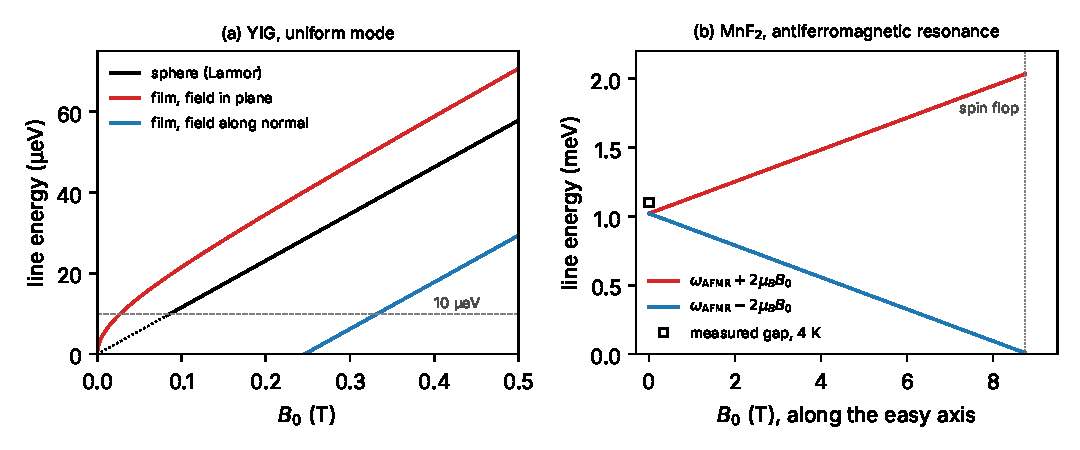
\includegraphics[width=0.95\linewidth]{figures/ch14/fig14_3.pdf}
  \caption{Absorption lines of YIG and MnF$_2$ against the applied field $B_0$. (a) The uniform mode of YIG ($g_{\mathrm{ion}} = 2$, $\mu_0M_{\mathrm{s}} = \SI{0.246}{T}$). A sphere absorbs at the Larmor frequency $2\mu_BB_0$ once it is saturated, $B_0 > \mu_0M_{\mathrm{s}}/3$ (dotted below). A thin film absorbs at $[\omega_{\mathrm{Lar}}(\omega_{\mathrm{Lar}} + \omega_M)]^{1/2}$ with the field in its plane and at $\omega_{\mathrm{Lar}} - \omega_M$ with the field along its normal, $\omega_M = \SI{28.5}{\micro eV}$. The dashed line marks the \SI{10}{\micro eV} of the worked example. (b) The two antiferromagnetic-resonance lines of MnF$_2$, $\omega_{\mathrm{AFMR}} \pm 2\mu_BB_0$ with $\omega_{\mathrm{AFMR}} = \SI{1.021}{meV}$ from $B_E = \SI{47.05}{T}$ and $B_A = \SI{0.82}{T}$, for a field along the easy axis up to the spin flop at \SI{8.75}{T}, both from the fitted fields; each line carries half of the weight $|\mathbf{S}|\omega_{\mathrm{AFMR}}/(2\omega_E + \omega_A) = 0.232$ per pair. The square is the measured zone-center gap at \SI{4}{K}, \SI{1.1}{meV}, which goes with a measured spin flop near \SI{9.4}{T}.}
  \label{fig:14-lines}
\end{figure}

\begin{limitbox}[Absorption into magnons][lim:14.3a]
(a) The Larmor statement: at $\vect{k} \to 0$ all transverse spin weight of a magnet with isotropic exchange and uniform $\lambda_S$ and $g_{\mathrm{ion}}$ lies in one line at $\omega_{\mathrm{Lar}}$ with weight $2\langle S^z_{\mathrm{tot}}\rangle$~\cites[Eqs.~(2.4), (2.5)]{oshikawa2002electron}[Eqs.~(25)--(27)]{chigusa2020detecting}[Eq.~(27)]{mitridate2020detectability}; for a $J$ multiplet the axion-like particle couples with $\lambda_S = g_J - 1$. (b) The uniform weight $|\vect{S}|\omega_{\mathrm{AFMR}}/(2\omega_E + \omega_A)$ per antiparallel pair, \cref{eq:14.3-afmrweight}.
\par\smallskip
{\centering
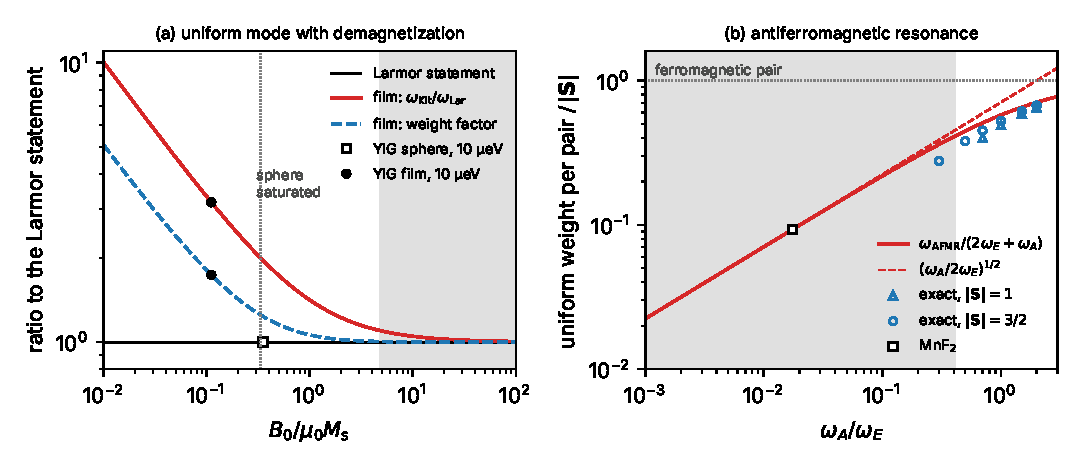
\includegraphics[width=0.98\linewidth]{figures/ch14/limit14_3a.pdf}
\captionof{figure}{(a) Uniform mode of a thin film with the field in its plane against the applied field over the shape-anisotropy field, $B_0/\mu_0M_{\mathrm{s}}$: line position $\omega_{\mathrm{Kit}}/\omega_{\mathrm{Lar}} = (1 + \mu_0M_{\mathrm{s}}/B_0)^{1/2}$ (solid) and weight averaged over transverse directions of $\vect{p}_\phi$ (dashed), both relative to the Larmor statement (black, 1). A saturated sphere follows the Larmor statement exactly; the markers place YIG at \SI{10}{\micro eV}. Gray: both ratios within \SI{10}{\percent} of 1, $B_0 \ge 4.8\,\mu_0M_{\mathrm{s}}$. For a $J$ multiplet both curves keep their shape, the rate scales by $(g_J - 1)^2$ and the line moves to $g_J\mu_BB_0$. (b) Uniform weight per antiparallel pair over $|\mathbf{S}|$ against $\omega_A/\omega_E$: the linear spin-wave result (solid) and its exchange-suppressed form $(\omega_A/2\omega_E)^{1/2}$ (dashed). Symbols: the exact total weight $\langle(S^x_{\mathrm{tot}})^2\rangle$ of the eight-site easy-axis (XXZ) cluster of the text for $|\mathbf{S}| = 1$ and $\frac32$, where that cluster is ordered (the splitting of its two lowest states below \SI{1}{\percent} of $\omega_{\mathrm{AFMR}}$). Gray: the square-root form within \SI{10}{\percent}, $\omega_A \le 0.42\,\omega_E$. The square marks MnF$_2$ with the fitted fields. The isotropic Heisenberg magnet, with zero uniform weight, is the left end.}\label{fig:14-limit-absorption}
\par}
\smallskip
Outside the gray regions the line of a non-spherical sample leaves $\omega_{\mathrm{Lar}}$ and its weight becomes elliptical, the antiferromagnetic weight departs from the square-root form, and in the eight-site cluster the zero-point fluctuations remove 5 to \SI{23}{\percent} of the linear spin-wave weight for $|\mathbf{S}| = \frac32$ ($\omega_A/\omega_E$ from 2 to 0.3).
\end{limitbox}

Linear spin-wave theory itself adds no correction to the Larmor line and one to the antiferromagnetic weight. \Cref{eq:14.3-larmor} is exact for any spin and temperature, and its only inputs are $\lambda_S$, $g_{\mathrm{ion}}$ and the net magnetization. The antiferromagnetic weight is of order $|\vect{S}|^0$ in the expansion of \cref{sec:14.1}, and an exactly solvable cluster shows its zero-point correction directly. Put spins $|\vect{S}|$ on the eight corners of a cube, each coupled to its three neighbors on the other sublattice by $H = J\sum_{\langle ij\rangle}(S^x_iS^x_j + S^y_iS^y_j + \Delta_{\mathrm{XXZ}}S^z_iS^z_j)$ with $J > 0$ and $\Delta_{\mathrm{XXZ}} \ge 1$, twelve bonds and open boundaries. Linear spin-wave theory at $\vect{k} = 0$ maps it onto \cref{eq:14.3-afmr} with $\omega_E = 3J|\vect{S}|$ and $\omega_A = 3J|\vect{S}|(\Delta_{\mathrm{XXZ}} - 1)$, so that \cref{eq:14.3-afmrweight} becomes $|\vect{S}|[(\Delta_{\mathrm{XXZ}} - 1)/(\Delta_{\mathrm{XXZ}} + 1)]^{1/2}$. The exact weight is the equal-time correlation $\langle0|(S^x_{\mathrm{tot}})^2|0\rangle$ in the ground state of the sector $S^z_{\mathrm{tot}} = 0$, divided by the four antiparallel pairs; it contains every final state that $S^x_{\mathrm{tot}}$ reaches. At $\omega_A = \omega_E$ it is 0.85 and 0.91 of \cref{eq:14.3-afmrweight} for $|\vect{S}| = 1$ and $\frac32$ (\cref{fig:14-limit-absorption}b). The cluster cannot reach the small anisotropies of real antiferromagnets, $\omega_A/\omega_E = 0.017$ in MnF$_2$, because below $\omega_A \approx 0.3\,\omega_E$ for $|\vect{S}| = \frac32$, and about $0.6\,\omega_E$ for $|\vect{S}| = 1$, its two lowest states mix and it no longer orders. For Mn$^{2+}$ the expansion parameter $1/2|\vect{S}|$ is 0.2, which sets the order of the correction at small $\omega_A/\omega_E$ but not its size.
